% Sketch output, version 0.3 (build 2d, Wed Apr 20 23:38:45 2011)
% Output language: PGF/TikZ,LaTeX
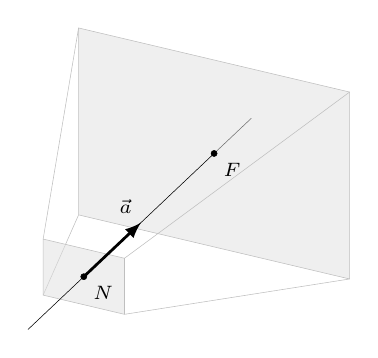
\begin{tikzpicture}[line join=round,line width=0.2pt,>=latex]
\draw[color=lightgray](.193,.437)--(.643,1.456);
\draw(2.364,2.236)--(2.837,2.683);
\filldraw[color=lightgray,fill=lightgray!50,fill opacity=0.5](4.085,3.016)--(.643,3.83)--(.643,1.456)--(4.085,.642)--cycle;
\draw[color=lightgray](.193,1.149)--(.643,3.83);
\draw(.709,.671)--(2.364,2.236);
\draw[color=lightgray](1.226,.193)--(4.085,.642);
\draw[color=lightgray](1.226,.905)--(4.085,3.016);
\filldraw[color=lightgray,fill=lightgray!50,fill opacity=0.5](1.226,.905)--(.193,1.149)--(.193,.437)--(1.226,.193)--cycle;
\draw(0,0)--(.709,.671);
\draw[->,line width=1pt](.709,.671)--(1.436,1.358);
\filldraw[](.709,.671) circle (1.1pt);
\filldraw[](2.364,2.236) circle (1.1pt);

    \coordinate [label=290:\scriptsize$N$] (N) at (.709,.671);
    \coordinate [label=290:\scriptsize$F$] (F) at (2.364,2.236);
    \coordinate [label=175:\scriptsize$\vec{a}$] (a) at (1.436,1.358);
  \end{tikzpicture}% End sketch output
